\documentclass[10pt,landscape]{article}
\usepackage[scaled=0.92]{helvet}
\usepackage{calc,multicol,ifthen}
\usepackage[a4paper,margin=5mm,landscape]{geometry}
\usepackage{amsmath,amsthm,amsfonts,amssymb,mathtools,bm}
\usepackage{color,graphicx,overpic,hyperref}
\usepackage{newtxtext}
\usepackage{enumitem}
\usepackage{braket}
\usepackage{physics}
\usepackage[table]{xcolor}
\usepackage{vwcol,tikz,nicematrix}
\usetikzlibrary{arrows.meta,calc}
\usepackage[T1]{fontenc}
\usepackage{cancel,mathrsfs,listings}
\setlist{nosep}
\lstset{language=Java,keywordstyle={\bfseries\color{black}}}
\pagestyle{empty}
\newenvironment{tightcenter}{\setlength\topsep{0pt}\setlength\parskip{0pt}\begin{center}}{\end{center}}
\makeatletter
\renewcommand{\section}{\@startsection{section}{2}{0mm}{-1ex plus -.5ex minus -.2ex}{0.5ex plus 0ex}{\normalfont\normalsize\bfseries}}
\renewcommand{\subsection}{\@startsection{subsection}{3}{0mm}{-1ex plus -.5ex minus -.2ex}{0.25ex plus 0ex}{\normalfont\small\bfseries}}
\renewcommand{\familydefault}{\sfdefault}
\renewcommand\rmdefault{\sfdefault}
\renewcommand{\labelenumii}{\theenumii}
\renewcommand{\theenumii}{\theenumi.\arabic{enumii}.}
\renewcommand\labelitemii{•}
\renewcommand{\lnot}{\mathord{\sim}}
\renewcommand{\bf}[1]{\textbf{#1}}
\newcommand{\Mod}[1]{\ \mathrm{mod}\ #1}
\newcommand{\uvec}[1]{\hat{\mathbf{#1}}}
\makeatother
\definecolor{myblue}{cmyk}{1,.72,0,.38}
\everymath\expandafter{\the\everymath \color{myblue}}
\newcommand{\vct}[1]{\bm{#1}}
\newcommand{\e}{\mathrm e}
\newcommand{\er}{\hat{\vct e}_r}
\newcommand{\et}{\hat{\vct e}_\theta}
\setcounter{secnumdepth}{0}
\setlength{\parindent}{0pt}
\setlength{\parskip}{0pt plus 0.5ex}
\setlength{\leftmargini}{0.5cm}
\setlength{\leftmarginii}{0.5cm}
\setlist[itemize,1]{leftmargin=2mm,labelindent=1mm,labelsep=1mm}
\setlist[itemize,2]{leftmargin=4mm,labelindent=1mm,labelsep=1mm}
\newtheorem{example}[section]{Example}
\begin{document}

\raggedright\footnotesize
\setlength{\columnseprule}{0.25pt}
\setlength{\premulticols}{1pt}
\setlength{\postmulticols}{1pt}
\setlength{\multicolsep}{1pt}
\setlength{\columnsep}{2pt}
\begin{multicols*}{4}

\begin{center}
    \fbox{%
        \parbox{0.8\linewidth}{\centering \textcolor{black}{
            {\Large\textbf{PC2032}}
            \\ \normalsize{AY26/27 Sem 1}}
            \\ {\footnotesize \textcolor{myblue}{by Boon How}} 
        }%
    }
\end{center}

% ====================================================
%                   Start Cheatsheet
% ====================================================

% ====================================================
%                      Chapter 1
% ====================================================

\section{1. Kinematics}
\subsection{Projectile Motion}
\begin{itemize}
    \item For constant $a$: 
    \begin{itemize}
        \item $v = v_0 + at$, $\quad x = x_0 + v_0t + \frac{1}{2}at^2$
        \item $v^2 = v_0^2 + 2a(x - x_0)$
    \end{itemize}
    \item For constant $\alpha$, replace $x$ with $\theta$, $v$ with $\omega$*
    \item Projectile: $x = x_0 + v_0\cos\theta\ t$, $\quad y = y_0 + v_0\sin\theta\ t - \frac{1}{2}gt^2$
\end{itemize}

\subsection{Circular Motion}
\begin{itemize}
    \item Tangential and radial components add up to the original acceleration: $\mathbf{a} = \mathbf{a}_r + \mathbf{a}_t$
    \begin{center}
        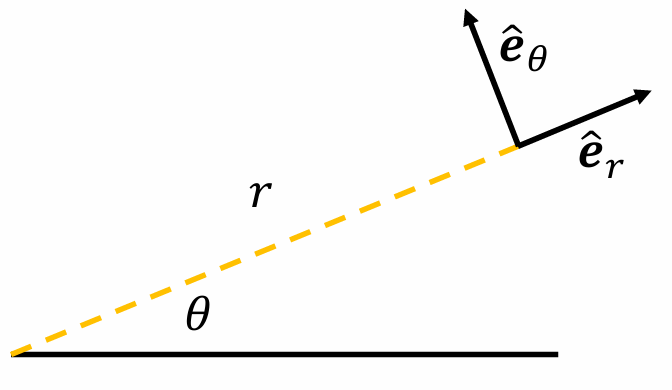
\includegraphics[width=0.4\linewidth]{images/kinematics polar coordinates.png}
    \end{center}
    \item $\dv{\uvec{e}_r}{t} = \dv{\theta}{t} \uvec{e}_\theta$, $\dv{\uvec{e}_\theta}{t} = -\dv{\theta}{t} \uvec{e}_r$
    \item Velocity: $\vb{v} = \dv{\vb{r}}{t} = \dv{t}(r \uvec{e}_r) = \dv{r}{t}\uvec{e}_r + r\dv{\uvec{e}_r}{t} = \dv{r}{t}\uvec{e}_r + r\dv{\theta}{t}\uvec{e}_\theta$
    \item Acceleration: $\vb{a} = \dv{\vb{v}}{t} = \left[ \dv[2]{r}{t} - r \left( \dv{\theta}{t} \right)^2 \right] \uvec{e}_r + \left[ r \dv[2]{\theta}{t} + 2 \dv{r}{t}\dv{\theta}{t} \right] \uvec{e}_\theta$
    \item For constant radius: 
    \begin{itemize}
        \item $\vb{v} = r\dv{\theta}{t}\uvec{e}_\theta = v\uvec{e}_\theta = r\omega\uvec{e}_\theta$
        \item $\vb{a} = -r \left(\dv{\theta}{t} \right)^2 \uvec{e}_r + r\dv[2]{\theta}{t}\uvec{e}_\theta = a_r\uvec{e}_r + a_t\uvec{e}_\theta$, where $a_r = -r \left(\dv{\theta}{t}\right)^2 = -r\omega^2 \text{ and } a_t = r\dv[2]{\theta}{t} = \alpha$
    \end{itemize}
    \item Uniform circular motion $\rightarrow$ constant speed and angular velocity: $\dv{\omega}{t} = \dv[2]{\theta}{t} = 0 \text{ , } \dv{r}{t} = 0$. Also, $\vb{a} = a\uvec{e}_r \text{ where } a = -r\omega^2 = -\frac{v^2}{r}$ is a constant
    \item For non-uniform circular motion, there will be non-zero tangential acceleration where $\vb{a}_t = a_t\uvec{e}_\theta $ and $ a_t = \dv{v}{t}$
    \item 3D description: we introduce angular velocity vector $\vb{\omega(t)}$. If we put origin on rotation axis, we get compact formula $\dot{\vb{r}} = \vb{\omega}(t) \cross \vb{r}(t)$ and $\abs{\vb{\omega}(t) \cross \vb{r}(t)} = \abs{\vb{\omega}(t)}s$, where s is the shortest distance to the axis
\end{itemize}

\subsection{Relative Motion}
\begin{itemize}
    \item Converting frame of reference: $\vb{r}_{P/B} = \vb{r}_{P/A} - \vb{r}_{B/A}$
    \item Differentiate further to get: $\vb{v}_{P/B} = \vb{v}_{P/A} - \vb{v}_{B/A}$ and $\vb{a}_{P/B} = \vb{a}_{P/A} - \vb{a}_{B/A}$
    \item For rotating frames with constant angular velocity, consider frame B rotating w.r.t frame A:
    \begin{itemize}
        \item No translational motion
        \item Rotation axis passes through origin
        \item Angular velocity vector $\vb{\Omega}$ is constant
    \end{itemize}
    Then, we have $\vb{a}_{P/B} = \vb{a}_{P/A} + \vb{a}_{\text{centrifugal}} + \vb{a}_{\text{Coriolis}}$
    \item Centrifugal acceleration has direction outward from rotation axis and magnitude $s\Omega^2$, where $s$ is shortest distance from rotation axis
    \item Coriolis acceleration: $\vb{a}_{\text{Coriolis}} = -2\vb{\Omega} \cross \vb{v}_{P/B}$
\end{itemize}

% ====================================================
%                      Chapter 2
% ====================================================

\section{2. Newtonian Physics}
\subsection{Centre of Mass and Extended bodies}
\begin{itemize}
    \item Applying Newton's second law to extended bodies, we get $\vb{F}_{\text{net external}} = \dv{\vb{p}_{\text{total}}}{t} = m\vb{a}_{\text{CM}}$
    \item \bf{Centre of Mass Formula}: $\vb{r}_{\text{CM}} = \frac{\int\vb{r}dm}{m_{\text{total}}} = \frac{\int \vb{r} \rho(\vb{r})dV}{m_{\text{total}}} = \frac{\int \vb{r} \rho(\vb{r})dV}{\int \rho(\vb{r})dV}$
    \item Use $\sigma dA$ for mass per unit area, $\lambda dL$ for mass per unit length. For circles, use $dV = 2\pi r\ dr$
    \item \bf{Centre of mass formula for 2 objects}: $\vb{r}_{\text{CM}} = \frac{M\vb{R} + m\vb{r}}{M + m}$, where $\vb{r}^{\text{rel}} = \vb{r} - \vb{R}$ ($r$ is vector from an origin!!)
    \item Circle polar coord: $x = r\cos\theta$, $y = r\sin\theta$, $r^2 = x^2 + y^2$, $dA = r\ dr\ d\theta$
    \item Sphere polar coord: $\rho^2 = x^2 + y^2 + z^2$, $x = \rho\sin\phi\cos\theta$, $y = \rho\sin\phi\sin\theta$, $z = \rho\cos\phi$, $dV = \rho^2\sin\phi\ d\rho\ d\phi\ d\theta$
\end{itemize}

\subsection{More Applications}
\begin{itemize}
    \item By definition, $F = -\dv{p}{t}$
    \item When an object is about to lose contact, normal force $N = 0$
    \item Tension and normal force can act as a constraint force, preventing object from passing through a surface.
    \item Hooke's law: $F_s = -kx$
    \item Spring in series: $\frac{1}{k_{\text{eff}}} = \frac{1}{k_1} + \frac{1}{k_2}$
    \item Static friction $f_s \leq \mu_sN$; Kinetic friction $f_k = \mu_kN$
    \item Generally, $\mu_k < \mu_s$
    \item Terminal speed kinematics: $\dv{v}{t} = g - \frac{k}{m}v$, $v = (mg/k)\left(1-e^{-kt/m}\right)$
    \item Air drag at high speeds: $mg - Dv^2 = ma$, terminal speed $v_t = \sqrt{mg/D}$
    \item Newton's first and second laws only hold in inertial frames. If we consider frames that are accelerated, we can introduce fictitious force $\vb{F}_{\text{fic}} = -m\vb{a}$ in the accelerated frame
    \item For rotating frames with angular velocity $\Omega$, introduce fictitious forces $\vb{F}_{\text{centrifugal}}$ with magnitude $ms\Omega^2$ directed outwards from rotation axis and $\vb{F}_{\text{Coriolis}} = -2m\Omega \cross \vb{v}_{P/B}$
\end{itemize}

% ====================================================
%                      Chapter 3
% ====================================================

\section{3. Energy}
\subsection{Energy and Work Done}
\begin{itemize}
    \item Work done $W = \int\vb{F}\cdot d\vb{x}$
    \item To compute the work done in a path, we compute the line integral of the path
    \item Work-Energy Theorem: work done = change in kinetic energy
    \item Power is energy per unit time and is denoted by $P = \vb{F} \cdot \dv{\vb{x}}{t} = \vb{F} \cdot \vb{v}$
    \item Similarly, $W = \int_P \vb{F} \cdot d\vb{x} = \int_{t_i}^{t_f} \vb{F} \cdot \dv{\vb{x}}{t} dt = \int_{t_i}^{t_f} P \ dt$
    \item Constraint forces generally act perpendicular to motion so they do no net work. Hence, we can ignore work done by constraint forces
\end{itemize}

\subsection{Conservation of Energy}
\begin{itemize}
    \item Conservative forces have these properties:
    \begin{itemize}
        \item Work done by $\vb{F}$ is path-independent
        \item Work done by $\vb{F}$ around any closed path is zero
        \item There exists scalar function $U$ such that $\vb{F} = -\nabla U$ (+ very mild assumptions)
    \end{itemize}
    \item Conservative force $F = -\dv{U}{x}$ is used for spring or gravitational potential energy
    \item Non-conservative forces include friction, resistive forces/drag and some electromagnetic effects    
    \item Potential energy property: $U(\vb{x}_2) - U(\vb{x}_1) = -\int_{\vb{x}_1}^{\vb{x}_2} \vb{F} \cdot d\vb{x}'$
    \item Potential energy of a spring is $U_{\text{spring}} = \frac{1}{2}kx^2$, where $x$ is displacement from "rest length" position
    \item Work-Energy, Extended Bodies Equation:
    \begin{center}
        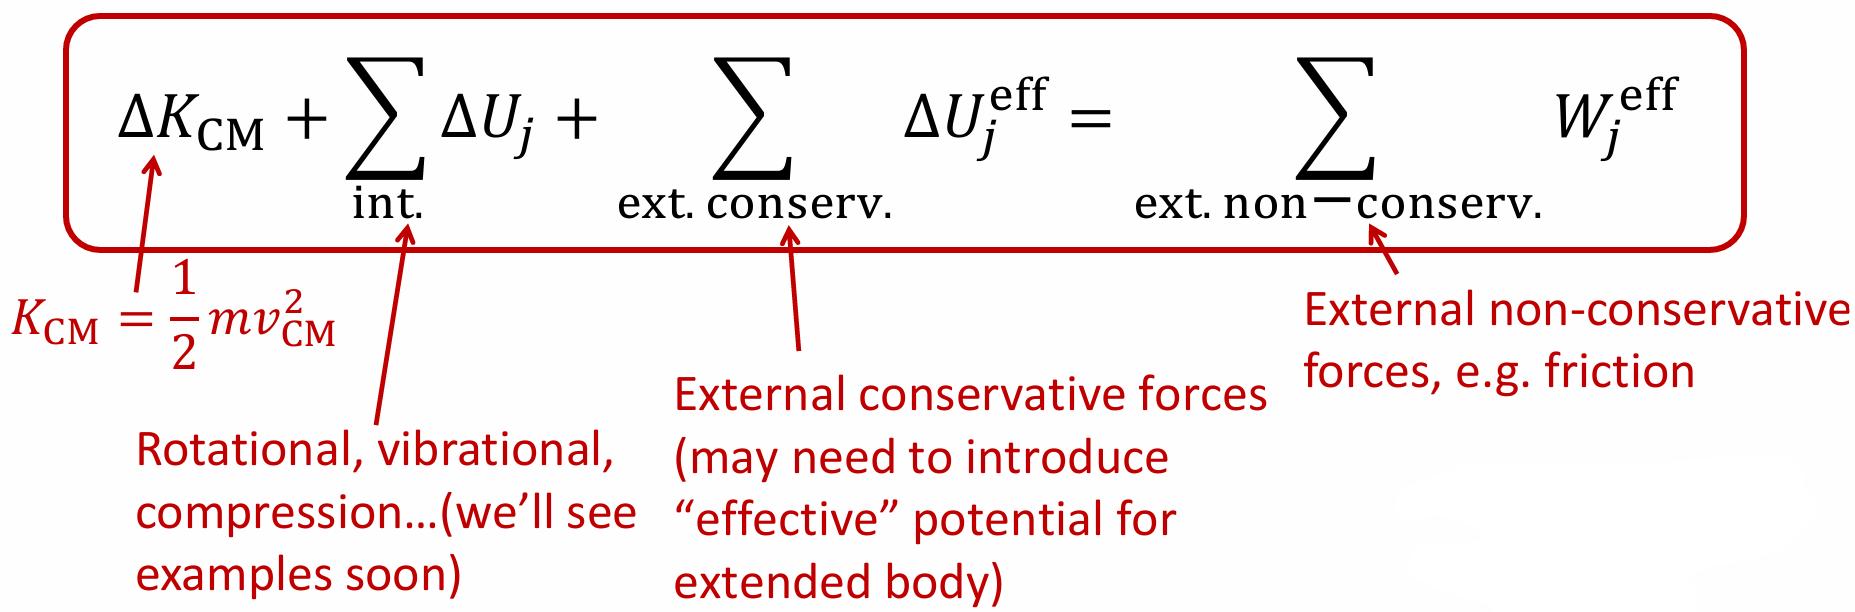
\includegraphics[width=1\linewidth]{images/work-energy, extended bodies.png}
    \end{center}
\end{itemize}

\subsection{Potentials}
\begin{itemize}
    \item For abstract $U(x)$, speed is $\abs{\dot{x}} = \sqrt{\frac{2(E-U)}{m}}$
    \item Simple harmonic motion formula can be generalized to $\ddot{q} = -\omega^2q$, where $q$ can be replaced with $\theta$ or $r$
    \item Note that $q$ is displacement of a coordinate from equilibrium, and is useful to substitute $q \coloneqq Q - Q^{\text{eq}}$
    \item Approximate harmonic motion uses Taylor expansion to obtain $\ddot{Q} \approx f'(Q^{\text{eq}})(Q - Q^{\text{eq}})$, or $\ddot{q} \approx f'(q^{\text{eq}})q$ for $q \coloneqq Q - Q^{\text{eq}}$
    \item For energy, as long as $U''(Q^{\text{eq}}) \neq 0$, we have $U(Q) \approx U(Q^{\text{eq}}) + \frac{U''(Q^{\text{eq}})}{2}(Q - Q^{\text{eq}})^2$
    \item By linearity, for more than 1 dimension, we can just add their potentials to study their behaviour. Doing so will give $U_{\text{total}}(\vb{r}) = -\int_{\text{origin}}^{\vb{r}} \vb{F}_{\text{total}} \cdot d\vb{r}$
    and $\vb{F}_{\text{total}} = - \nabla U_{\text{total}}$
\end{itemize}

% ====================================================
%                      Chapter 4
% ====================================================

\section{4. Momentum}
\subsection{Collisions}
\begin{itemize}
    \item Conservation of momentum (CoM) states that if net external force is zero, total momentum is constant, i.e. $\vb{p}_i = \vb{p}_f$
    \item We can also regroup the particles to write $\vb{p}_{\text{total}} = m_{\text{total}}\vb{v}_{\text{CM}}$
    \item In CM frame, total momentum is always zero if net external force is zero
    \item Impulse ($\Delta\vb{p}$) $\vb{J} = \int_{t_i}^{t_f} \vb{F}_{\text{net}}\ dt$ , where $\vb{F}_{\text{net}} = \dv{\vb{p}}{t}$
    \item Angular impulse $\Delta L = \int \tau\ dt$; $Jh = I_{\text{CM}}\omega$
    \item Common classifications for collisions:
    \begin{itemize}
        \item \bf{Elastic} collision: both momentum and KE conserved
        \item \bf{Inelastic} collision: momentum conserved, KE not conserved; \bf{Perfectly inelastic} collision: particles \bf{"stick together"}, so they have the same final velocity
    \end{itemize}
    \item Conservation of momentum (doesnt work when theres torque, use CoAM instead): $m_1v_{1i} + m_2v_{2i} = m_1v_{1f} + m_2v_{2f}$
    \item Conservation of (kinetic) energy: $m_1v_{1i}^2 + m_2v_{2i}^2 = m_1v_{1f}^2 + m_2v_{2f}^2$
    \item For 1D elastic collisions, $v_{1f} = \left(\frac{m_1 - m_2}{m_1 + m_2}\right)v_{1i} + \left(\frac{2m_2}{m_1 + m_2}\right)v_{2i}$; $v_{2f} = \left(\frac{2m_1}{m_1 + m_2}\right)v_{1i} + \left(\frac{m_1 - m_2}{m_1 + m_2}\right)v_{2i}$
    \item For 1D perfectly inelastic collisions, $v_f = \frac{m_1v_{1i} + m_2v_{2i}}{m_1 + m_2} = v_{\text{CM}}$. This formula applies to higher dimensions as well (just replace $v$ with $\vb{v}$)
    \item For 2D collisions, apply conservation of momentum for $x$ and $y$ components
    \item For 3D collisions, find a plane such that the $z$-component of both particles' paths align, then solve it like the 2D case
\end{itemize}

\subsection{Variable Mass}
\begin{itemize}
    \item Rocket Science:
    \begin{center}
        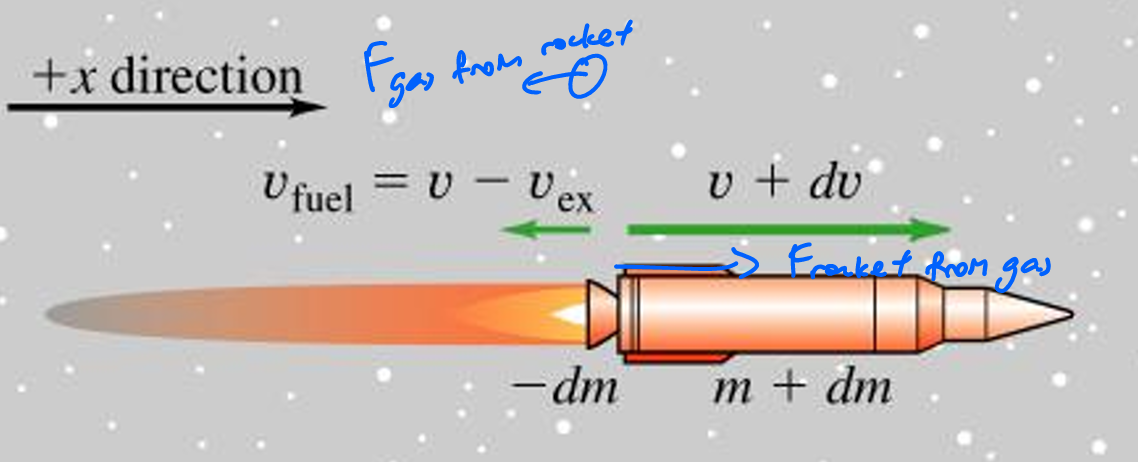
\includegraphics[width=0.5\linewidth]{images/rocket.png}
    \end{center}
    \item At time $t$,
    \begin{itemize}
        \item $m$: mass of rocket (note: this mass is changing)
        \item $v$: velocity of rocket (space frame)
    \end{itemize}
    \item At time $t + dt$,
    \begin{itemize}
        \item $m + dm$: mass of rocket ($dm < 0$)
        \item $v + dv$: velocity of rocket (space frame)
        \item $-dm$: mass of gas (note: $-dm > 0$)
        \item $v_{\text{fuel}}$: velocity of gas (space frame, so $v_{\text{fuel}} = v - u_{\text{ex}}$)
    \end{itemize} 
    Momentum at $t + dt$: $(m + dm)(v + dv) + (-dm)(v - u_{\text{ex}})$
    \\ Momentum at $t$: $mv$
    \\ No external forces so $p_{\text{total}}$ is constant, $\Delta p = 0$
    \\ After solving, we get: $v_f - v_i = u_{\text{ex}}\ln(m_i/m_f)$
    \\ note: in the process we get $dmdv \approx 0$ which is negligible
    \item If all exhaust exhausted at once, 
    \\Transform to frame where $v_i = 0$:
    \\ $m_fv_f = -(m_i-m_f)(v_f-u_{\text{ex}})$
    \\ Transform back: $v_f - v_i = \left(1 - \frac{m_f}{m_i}\right) u_{\text{ex}}$
\end{itemize}

% ====================================================
%                      Chapter 5
% ====================================================

\section{5. Rotational Mechanics}
\subsection{Rigid-Body Kinematics}
\begin{itemize}
    \item Often useful to consider positions of point masses relative to some point $\vb{r}_j^{\text{rel}}(t) = \vb{r}_j(t) - \vb{R}(t)$
    \item Rigid body is a set of point masses where distance between every pair of points must remain constant. Also, for every vector $\vb{\gamma}(t)$ of constant magnitude, $\vb{\dot{\gamma}} \perp \vb{\gamma}$
    \item For relative velocities between points at constant distance: $\vb{\dot{r}}_j^{\text{rel}}(t) \perp \vb{r}_j^{\text{rel}}(t)$
    \item Rigid body motion: $\vb{\dot{r}}_j^{\text{rel}}(t) = \vb{\omega}^{\text{rel}}(t) \cross \vb{r}_j^{\text{rel}}(t)$
    \item If we have relative instantaneous rotation: $\vb{\dot{r}}_j(t) = \vb{\dot{R}}(t) + \vb{\omega}^{\text{rel}}(t) \cross \vb{r}_j^{\text{rel}}(t)$ (velocity + pure rotation)
    \begin{center}
        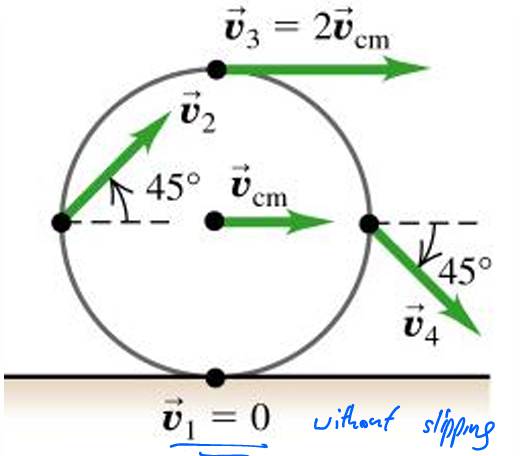
\includegraphics[width=0.4\linewidth]{images/rolling without slipping.png}
    \end{center}
    \item For rolling without slipping, $s = R\theta$
    \begin{itemize}
        \item $v_{\text{CM}} = R\omega$
        \item $a_{\text{CM}} = R\dv{\omega}{t} = R\alpha$. We also have $a = \frac{F}{M + I/R^2}$ for $F$ applied through CM
    \end{itemize}
    \item For rolling without slipping down an incline, $a_{\text{CM}} = \frac{g\sin\theta}{1 + \frac{I_{\text{CM}}}{MR^2}}$
    \item For rolling on incline under gravity alone, $f_s = \frac{k}{1 + 1/k}Mg\sin\theta$, where $k = \frac{I}{MR^2}$
    \item Since bottom-most point is stationary relative to surface, there is static friction but not kinetic friction, and static friction does no net work so it doesn't affect work-energy theorem
    \item For rolling in general, we may have $V_{\text{centre}} \neq R\omega$. So, it has kinetic friction instead of static friction and contact points of object and surface are not stationary w.r.t. each other
\end{itemize}

\subsection{Inertia and Energy}
\begin{itemize}
    \item (scalar) Moment of inertia, $I = \sum_j m_j s_j^2$
    \item Kinetic energy, $K_{\text{total}} = \frac{1}{2}I\omega^2$
    \item Moments of inertia can add up, i.e. $I_{\text{combined}} = I_1 + I_2$ (can use with parallel-axis theorem to find MOI of a system)
    \item For "continuous" bodies with density $\rho$, $I = \int s^2\ dm = \int \rho s^2 \ dV$. Use $\sigma \ dA$ or $\lambda \ dL$ instead for 2D or 1D
    \item Parallel-Axis Theorem: $I = m_{\text{total}}s_{\text{CM}}^2 + I_{\text{CM}}$, $s_{\text{CM}}$ is CM perpendicular (shortest) distance from axis, $I_{\text{CM}}$ is MOI about the parallel axis that passes through CM
    \item  Perpendicular-Axis Theorem (only work on 2D bodies):
    \begin{itemize}
        \item For any 2 perpendicular axes in the plane of the body, with moments of inertia $I_x$, $I_y$, intersecting at a point $P$,
        \item Moment of inertia $I_z$ about axis through $P$, perpendicular to plane of body, will be $I_z = I_x + I_y$
    \end{itemize}
    \item Important property: $\sum_j m_j \vb{r}_{j}^{\text{rel}} = 0$, i.e. "mass-weighted sum" of relative positions is zero
    \item Kinetic Energy Decomposition: $K_{\text{CM}} = \frac{1}{2}m_{\text{total}}\abs{\vb{\dot{R}}_{\text{CM}}}^2$; $K_{\text{int}} = \frac{1}{2} \sum_j m_j \abs{\vb{\dot{r}}_j^{\text{rel}}}^2$
    \item \bf{Warning}: only works for $R_{\text{CM}}$ (needs $\sum_j m_j \vb{r}_{j}^{\text{rel}} = 0$ trick)
    \item Kinematic Energy Decomposition (Rigid Body):
    \begin{itemize}
        \item $K_{\text{int}} = \frac{1}{2}\sum_j m_j \abs{\vb{\dot{r}}_j^{\text{rel}}}^2 = \frac{1}{2}\sum_j m_j \abs{\vb{\omega}^{\text{rel}} \cross \vb{r}_j^{\text{rel}}}^2 = \frac{1}{2} I_{\text{CM}}(\omega^{\text{rel}})^2$
        \item where $I_{\text{CM}} = \sum_j m_j \abs{s_j^{\text{rel}}}^2$ is a MOI about an axis through CM
    \end{itemize}
\end{itemize}

\subsection{Torque and Angular Momentum}
\begin{itemize}
    \item Angular Momentum, $\vb{L} = \vb{r} \cross \vb{p} = m\vb{r} \cross \vb{v} = m\vb{r} \cross \vb{\dot{r}}$
    \item $L_{\text{total}} = I\omega$; $L^z = ms^2\dot{\theta}$
    \item $\vb{r} \cross \vb{v} = v^{\tan}s \uvec{k}$, where $v^{\tan} = \dot{\theta}s$ is tangential velocity component, and $s$ is distance from origin
    \item Angular Momentum Decomposition: $\vb{L}_{\text{total}} = \vb{L}_{\text{CM}} + \vb{L}_{\text{int}}$, where $\vb{L}_{\text{CM}} = \vb{R}_{\text{CM}} \cross m_{\text{total}}\vb{\dot{R}}_{\text{CM}}$ ("Centre of mass angular momentum"), $\vb{L}_{\text{int}} = \sum_j \vb{r}_j^{\text{rel}} \cross m_j\vb{\dot{r}}_j^{\text{rel}}$ ("Internal angular momentum")
    \item Torque, $\vb{\tau}^{\text{net external}} = \dv{\vb{L}_{\text{total}}}{t} = \underset{j}{\sum}\vb{r}_j \cross \vb{F}_j^{\text{net external}}$
    \item Taking z-component of torque, $\tau^z \uvec{k} = \vb{r}_{\text{proj}} \cross \vb{F}_{\text{proj}}$, where $\vb{r}_{\text{proj}} \perp \vb{F}_{\text{proj}}$
    \item If everyting is stationary, i.e. velocities are zero, $\vb{F}^{\text{net external}} = \dv{\vb{p}_{\text{total}}}{t} = 0$ and $\vb{\tau}^{\text{net external}} = \dv{\vb{L}_{\text{total}}}{t} = 0$
    \item When torque is zero, $\vb{L}_{\text{total}} = 0$, angular momentum is conserved. Use CoAM as well when introducing new object approaching at constant velocity
    \item For pure rotation of a rigid body, $\tau_{\text{net external}}^z = I \dv{\omega^z}{t} = I\alpha$, where $\alpha$ is the angular acceleration
\end{itemize}

% ====================================================
%                      Chapter 6
% ====================================================

\section{6. Lagrangian Mechanics}
\subsection{Euler-Lagrange Equations}
\begin{itemize}
    \item Lagrangian $\mathcal{L} = T - V$, where $T = \frac{1}{2}m\dot{x}^2$ is KE, and $V$ is potential energy
    \item Principle of Stationary Action: Of all possible paths connecting the same initial and final configurations at fixed times, the actual path is one for which the action does not change to first order under a small variation of the path (i.e. $\delta S = 0$)
    \item Action, $S = \int_{t_i}^{t_f} \mathcal{L} \ dt = \int_{t_i}^{t_f} (T - V) \ dt$
    \item We assume that if the particle(s) are described by coordinates ${q_j(t)}$, $\mathcal{L}$ is only a function of these $q_j$, their first time derivatives, and time: $\mathcal{L} = \mathcal{L}(q_j, \dot{q}_j, t)$
    \item If some trajectory(s) give a stationary point of action, then it satisfies the \bf{Euler-Lagrange Equation}: $\dv{t}\left(\pdv{\mathcal{L}}{\dot{q}_j}\right) = \pdv{\mathcal{L}}{q_j}$
    \item If we set $\mathcal{L}(q_j, \dot{q}_j, t) = T - V$, then particles will follow trajectories s.t. $\int_{t_i}^{t_f} \mathcal{L}(q_j, \dot{q}_j, t) \ dt$ is a stationary point, which also implies the Euler-Lagrange equation hold
    \item When the qn ask for equations of motion, it suffice to show the differential equations involving the respective coordinates
\end{itemize}

\subsection{Noether's Theorem}
\begin{itemize}
    \item Noether's Theorem: every "continous symmetry" in a physical system corresponds to a conserved quantity, and vice versa \\
    \begin{center}
        $\mathcal{L}$ has no "explicit" dependence on coordinate $q_j$ \\
        $\Leftrightarrow \dv{t}\left(\pdv{\mathcal{L}}{\dot{q}_j}\right) = \pdv{\mathcal{L}}{q_j} = 0$ \\
        $\Leftrightarrow \pdv{\mathcal{L}}{\dot{q}_j}$ is a conserved quantity
    \end{center}
    \begin{itemize}
        \item Independent of Cartesian coord $r_j \Leftrightarrow$ translation symmetry along that direction $\Leftrightarrow$ conservation of linear momentum
        \item Independent of Angular coord $\theta \Leftrightarrow$ rotation symmetry w.r.t. an axis $\Leftrightarrow$ conservation of angular momentum w.r.t. that axis
    \end{itemize}
    \item Such a coordinate $q_j$ is called a cyclic coordinate
    \item When $\mathcal{L}$ has no "explicit" time dependence, $\pdv{\mathcal{L}}{t} = 0 \Leftrightarrow \underset{j}{\sum}\left(\pdv{\mathcal{L}}{\dot{q}_j} \dot{q}_j\right) - \mathcal{L} = \text{const}$
\end{itemize}

% ====================================================
%                      Chapter 7
% ====================================================

\section{7. Central Forces}
\begin{itemize}
    \item Central force $\vb{F} = f(r)\uvec{r}$, where $f(r)$ is a function of (only) distance $r$ from origin, always points towards the origin
    \item Since torque exerted by central force is $\vb{\tau} = \vb{r}\cross\vb{F} = \vb{r}\cross f(r)\uvec{r} = 0$, angular momentum is always conserved
    \item Central forces are conservative. Note: This only require $U(r)$ to be an indefinite integral of $f(r)$, i.e. $U(r) = \int f(r) \ dr$
    \item Suppose $U(r)$ is the potential for central force; use polar coords $(r, \theta)$ in the plane of motion: $\mathcal{L} = \frac{1}{2}m(\dot{r}^2 + r^2\dot{\theta}^2) - U(r)$
    \item $\theta$ is a cyclic coordinate $\Rightarrow \pdv{\mathcal{L}}{\dot{\theta}}$ is a conserved quantity
    \item Resulting equations:
    \[
    \begin{aligned}
        m\ddot{r} &= \frac{L^2}{mr^3} - U'(r) = -U'_{\text{eff}}(r), \\
        U_{\text{eff}}(r) &\coloneqq \frac{L^2}{2mr^2} + U(r),
    \end{aligned}
    \]
    where $\frac{L^2}{2mr^2}$ is the "angular momentum barrier"; radial coord $r$ behaves like 1D motion under eff. potential $U_{\text{eff}}(r)$
    \item Total energy $E$ is also conserved: $\frac{1}{2}m\dot{r}^2 + U_{\text{eff}}(r) = E$ (or $m\ddot{r} = -U'_{\text{eff}}(r)$) for $r$
    \item If we want the "shape" of the particle in space, $\frac{1}{r^4}\left(\dv{r}{\theta}\right)^2 = \frac{2m(E - U_{\text{eff}}(r))}{L^2}$ 
    \item Example: Inverse-Square Force (Attractive)
    \begin{center}
        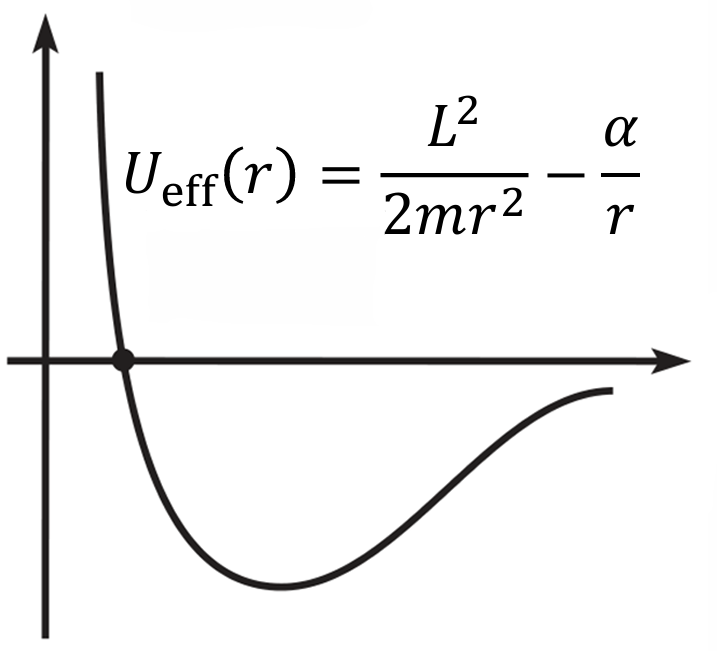
\includegraphics[width=0.35\linewidth]{images/inverse square law attractive.png}
    \end{center}

    \item When $E \geq 0$, we get \textbf{unbound} orbits/trajectories
    \item When $E < 0$, we get \textbf{bound} orbits/trajectories
    \item When $E = \text{min value of }U_{\text{eff}}$ (which is $-\frac{m\alpha^2}{2L^2}$)
    \begin{itemize}
        \item $r$ remains constant at equilibrium
        \item Particle in circular orbit $\Leftrightarrow \abs{\text{centripetal force}} = \abs{f(r)} = \abs{U'(r)}$
        \item If slightly perturbed, the orbit become ellipse shaped
    \end{itemize}
    \item Two-Body Problem: trick is to consider one particle's frame of reference
    \begin{itemize}
        \item Consider two object with mass $M$ and $m$
        \item In $M\text{'s}$ frame, $m\text{'s}$ acceleration is $\frac{\vb{F}}{m} - \frac{-\vb{F}}{M} = \left(\frac{m + M}{mM}\right)\vb{F}$
        \item Hence, we can rewrite $\ddot{r}^{\text{rel}} = \frac{\vb{F}}{\mu}$, where $\mu = \frac{mM}{m + M}$ and $\mu$ is called reduced mass (also always $< m$)
    \end{itemize}
    \item CM + relative position: given $\vb{r}_{\text{CM}}$ and $\vb{r}^{\text{rel}}$, recall:\\ 
    \begin{center}
        $\vb{r}_{\text{CM}} = \frac{M\vb{R} + m\vb{r}}{M + m}, \qquad \vb{r}^{\text{rel}} = \vb{r} - \vb{R}$
    \end{center}
    We can solve it algebraically to get $r$ and $R$
\end{itemize}

% ====================================================
%                      Chapter 8
% ====================================================

\section{8. Gravity}
\subsection{Newtonian Formulation}
\begin{itemize}
    \item Newton's Law of Universal Gravitation: $\abs{\vb{F}_g} = \frac{Gm_1m_2}{r^2}$, where $G = (6.67 \pm 0.01)\cross 10^{-11}\ \text{Nm}^2\ \text{kg}^{-2}$
    \item Gravitational Potential Energy: $U_g(r) = -\frac{GMm}{r}$
    \item Example: Thin Uniform Ring
    \begin{center}
        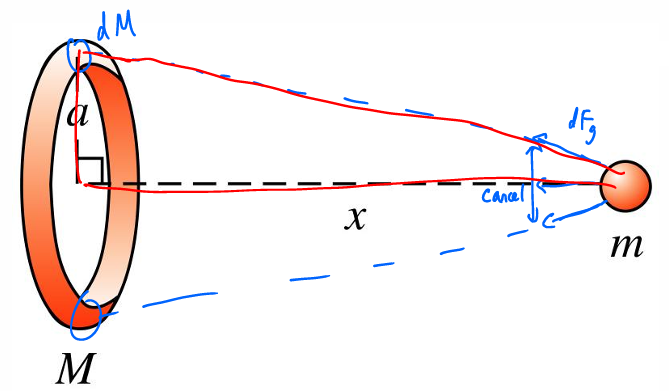
\includegraphics[width=0.5\linewidth]{images/thin uniform ring.png}
    \end{center}
    \begin{center}
            $\abs{d\vb{F}_g}\frac{x}{\sqrt{x^2 + a^2}} = \frac{Gmx \ dM}{(x^2 + a^2)^{3/2}}$ \\
            $\abs{\vb{F}_g^{\text{horizontal}}} = \int_{\text{ring}} \frac{Gmx \ dm}{(x^2 + a^2)^{3/2}} = \frac{GMmx}{(x^2 + a^2)^{3/2}}$
    \end{center}
    \item Shell Theorem (for thin uniform sphere):
    \begin{itemize}
        \item Outside the sphere: $F_g = -\frac{GMm}{r^2}\uvec{r}$ (same as a point mass at centre)
        \item Inside the sphere: zero
    \end{itemize}
    \item For solid uniform ball
    \begin{itemize}
        \item Outside the ball: (e.g. point $P$), $\vb{F}_g = -\frac{GMm}{r^2}\uvec{r}$
        \item Inside the ball (e.g. point $Q$), mass $M' = M\left(\frac{r}{R}\right)^3$, thus $\vb{F}_g = -\frac{GM'm}{r^2}\uvec{r} = -\frac{GMmr}{R^3}\uvec{r}$
    \end{itemize}
    \begin{center}
        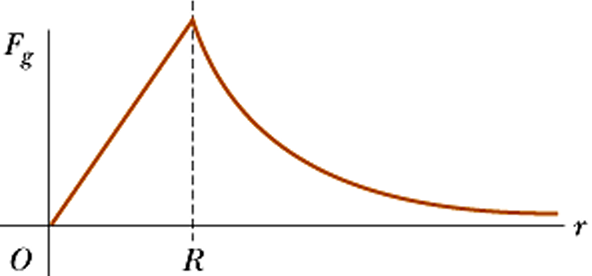
\includegraphics[width=0.4\linewidth]{images/solid uniform ball graph.png}
    \end{center}
    \item When computing the GPE of a collection of point masses, we only count each pair once, e.g. if we have 4 point masses: $U = U_{12} + U_{13} + U_{14} + U_{23} + U_{24} + U_{34}$
\end{itemize}

\subsection{Astronomical Bodies, Orbits}
\begin{itemize}
    \item Escape velocity: $v_i \geq v_{\text{esc}} = \sqrt{2GM/R}$
    \item Schwarzschild Radius: For a given $M$, can solve for critical $R$ at which it would be a black hole is $R_S = \frac{2GM}{c^2}$
    \begin{center}
        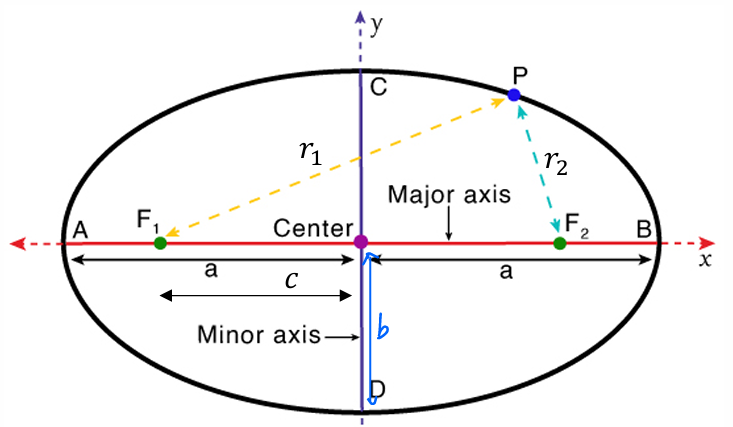
\includegraphics[width=0.6\linewidth]{images/ellipse.png}
    \end{center}
    \item Some properties for ellipse:
    \begin{itemize}
        \item If $a > b$, we call them semi-major axis $a$ and semi-minor axis $b$
        \item For 2 foci of equal distances from the center $F_1 \And F_2$, the sum of distances from the foci to any point on ellipse is constant: $r_1 + r_2 = 2a$ (can be found by placing point $P$ at point $B$)
        \item Eccentricity $e = c/a$
        \item Area $A = \pi ab$
        \item In suitable coordinates, described by equation $x^2/a^2 + y^2/b^2 = 1$
    \end{itemize}
    \item Conic sections: intersections between a plane and a pair of cones
    \begin{center}
        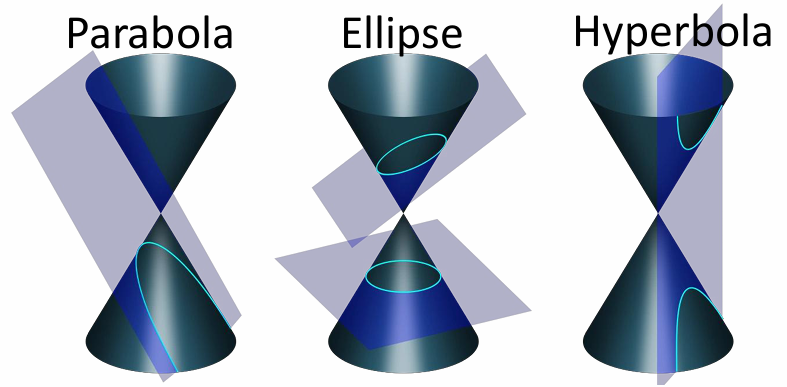
\includegraphics[width=0.5\linewidth]{images/conic sections.png}
    \end{center}
    \item Properties of hyperbolas: approaches 2 "linear asymptopes"; described by equation $x^2/a^2 - y^2/b^2 = 1$
    \item Kepler's First Law:
    \begin{itemize}
        \item At perihelion and aphelion, $\vb{r} \perp \vb{v}$
        \item When $e = 0$, we have a circle
        \item When $e \rightarrow 1$, it approaches a "flat" ellipse
    \end{itemize}
    \item Kepler's First Law, Extended:
    \begin{itemize}
        \item Solve DE for attractive inverse-square central force $\vb{\ddot{r}} = -\frac{GM}{r^2}\vb{r}$
        \item All solutions of this DE are conic sections (except trivial case where angular momentum $L = 0$)
        \item $K + U < 0$ ellipses (bound orbits)
        \item $K + U > 0$ hyperbola (unbound "orbits", approaches constant-velocity motion)
        \item $K + U = 0$ parabola (just "barely" unbounded: $v_{\text{esc}}$ is one example)
    \end{itemize}
    \item Kepler's Second Law: equal areas swept out in equal times (CoAM in disguise). Calculating the area of triangle, we get $dA = \frac{1}{2}r(rd\theta) \Rightarrow \dv{A}{t} = \frac{1}{2}r^2\dv{\theta}{t} = \frac{L}{2m}$
    \item Kepler's Third Law: $T^2 = \frac{4\pi^2a^3}{GM}$
\end{itemize}

\end{multicols*}
\end{document}